\chapter{Detalles de Implementación y Resultados}\label{chapter:implementation}

Siguiendo el proceso de investigación descrito en el capítulo anterior, 
en el presente se detallará la implementation de dicho proceso. 

\section{Construcción del conjunto de datos}

Para la creación de los datasets se utilizó Python 3.10 como lenguaje de programación. 
Este lenguaje cuenta con la característica de poseer muchas librerías de gran utilidad en el análisis y manejo de datos. Las utilizadas 
en este estudio para la recopilación y el procesamiento de los datos son: \texttt{pandas} y \texttt{requests}.  

La librería \texttt{pandas} es ampliamente utilizada cuando se trabaja con grandes volúmenes de datos, también para el manejo de archivos .xlsx. 
Los principales tipos de datos en esta librería son: \texttt{DataFrame} y \texttt{Series}. Para esta investigación se empleó fundamentalmente 
el tipo de dato \texttt{DataFrame} el cual modela el funcionamiento de una hoja de trabajo en excel. El archivo de registros de Moodle se procesó con esta librería, 
mediante el método \texttt(extract()) se transformó la columna de "Descripción" por tres nuevas columnas (ID\_USUARIO, ID\_MODULO, ID\_CURSO).  


La librería \texttt{requests} se utiliza para hacer las peticiones al API de Moodle. Estas se realizan a partir de un token y una url proporcionadas por la institución en cuestión.  

\begin{figure}
    \centering
    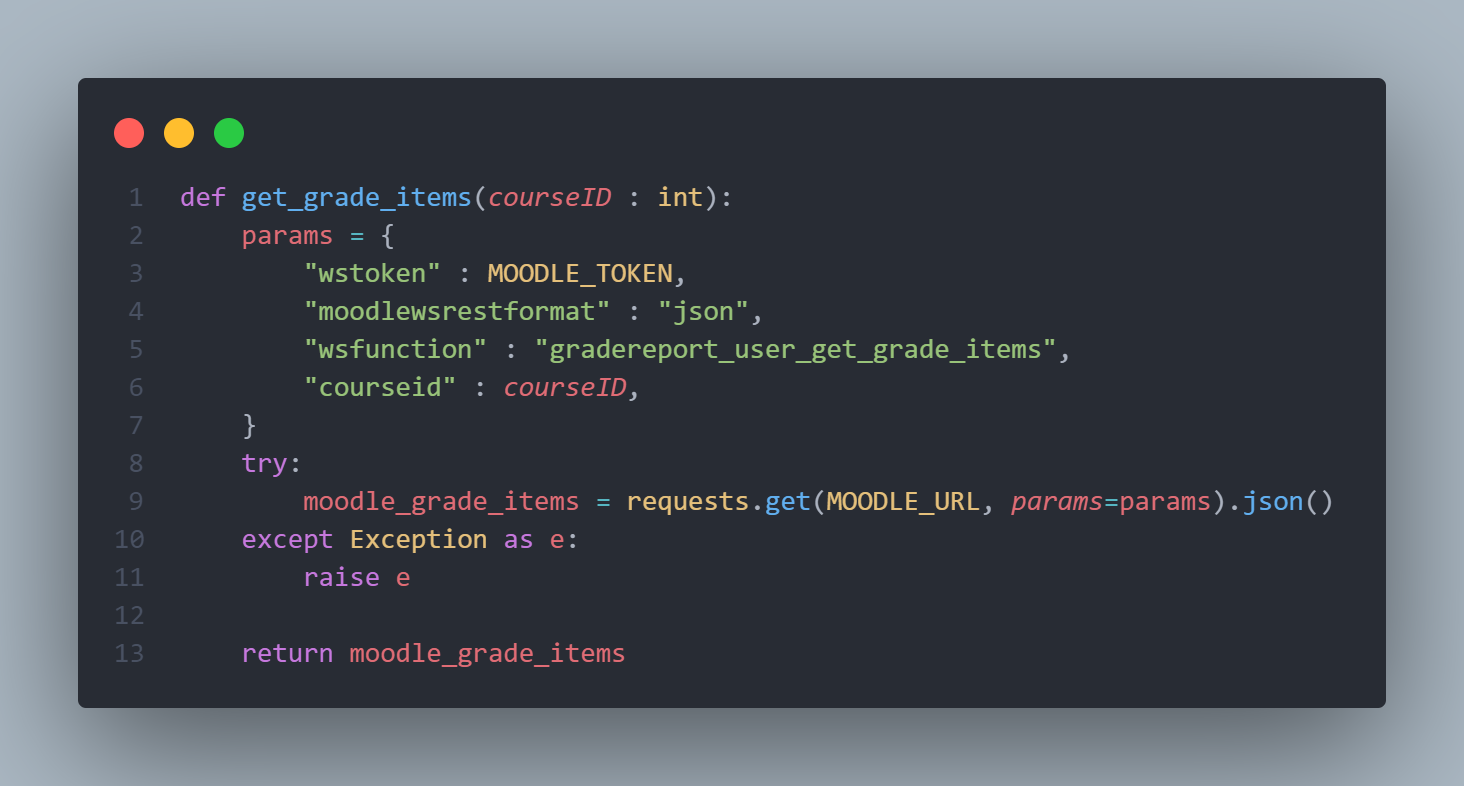
\includegraphics[width = 1 \textwidth]{Graphics/code.png}
    \caption{Ejemplo de código para el llamado al API de Moodle}
    \label{ApiMoodle}
\end{figure}

En la figura \ref{ApiMoodle} se presenta un ejemplo de un método que obtiene el libro de calificaciones de un curso en Moodle a través del API. 

Una vez procesado el archivo de registros y fusionado con las calificaciones de los estudiantes, se obtienen los datasets que se presentan en las figuras \ref{dataset1_view} y \ref{dataset2_view}.  


\begin{figure}
    \centering
    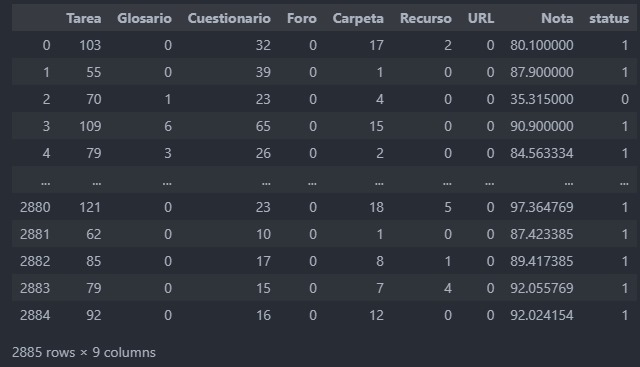
\includegraphics[width = 1 \textwidth]{Graphics/dataset1_view.jpg}
    \caption{Muestra del \textit{Dataset} 1}
    \label{dataset1_view}
\end{figure}

\begin{figure}
    \centering
    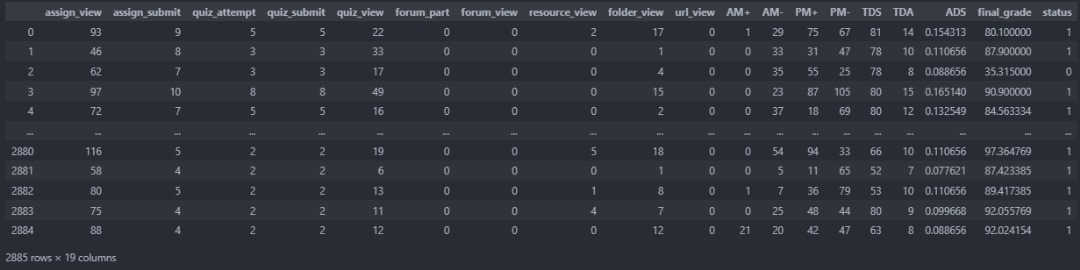
\includegraphics[width = 1 \textwidth]{Graphics/dataset2_view.jpg}
    \caption{Muestra del \textit{Dataset} 2}
    \label{dataset2_view}
\end{figure}  


A partir del campo \textbf{Fecha}, que se encuentra en el archivo de registros de Moodle, se dividieron ambos \textit{datasets} en 4 (25\%, 50\%, 75\%, 100\%). Para la selección de características 
se empleó el conjunto de datos que contiene el 100\% en cada caso. Para tener una mejor apreciación de cómo se comportan las características seleccionadas en ambos \textit{datasets} se calculó la 
Matriz de Correlación, y se realizó un proceso de selección de características con el algoritmo \textbf{Boruta}.  

La Matriz de Correlación es una herramienta estadística que muestra la intensidad y la dirección de la relación entre dos o más variables. Muestra cómo se relacionan entre sí todos los posibles 
pares de valores de una tabla con el coeficiente de correlación. Este oscila entre -1 y 1, donde -1 significa una correlación negativa perfecta, 
1 significa una correlación positiva perfecta y 0 significa que no hay correlación entre las variables. El coeficiente de correlación se calcula a partir de la siguiente fórmula: 

\begin{center}
    $r = \frac{n\sum{XY}}{\sqrt{(n\sum{X^2}-(\sum{X})^2)(n\sum{Y^2} - (\sum{Y})^2)}}$
\end{center}

Donde : 

\begin{itemize}
    \item $r =$ coeficiente de correlación
    \item $n =$ número de observaciones
    \item $\sum{XY} =$ suma del producto de cada par de observaciones correspondientes de las dos variables
    \item $\sum{X} =$ suma de las observaciones de la primera variable
    \item $\sum{X^2}$ = suma de los cuadrados de las observaciones de la primera variable
    \item $\sum{Y^2}$ = suma de los cuadrados de las observaciones de la segunda variable  
\end{itemize}

Esta matriz hace que sea fácil y rápido observar cómo están relacionadas las distintas variables y de esta forma encontrar patrones en ellas.  

Se construyeron Modelos de Aprendizaje automático con este \textit{dataset} en las cuatro etapas del curso. El lenguaje de programación utilizado fue con la librería textit{scikit-learn} en su versión 1.3.2, a través de Google Colab, una plataforma 
de código abierto que admite muchas bibliotecas populares de aprendizaje automático, entre ellas \textit{scikit-learn}. [\cite{wei-meng2019python}].  

Se crearon y ejecutaron 5 clasificadores binarios con parámetros predeterminados, como Árbol de Decisión, \textit{Random Forest}, 
Regresión Logística, Regresión Lineal, \textit{Support Vector Machine}. Estos modelos se entrenan en las diferentes etapas de un curso, una primera vez con todas los 
atributos y luego con un filtro de características a partir del resultado del algoritmo Boruta.


\subsection{Análisis del primer \textit{dataset}}

\begin{figure}[htb]
    \centering
    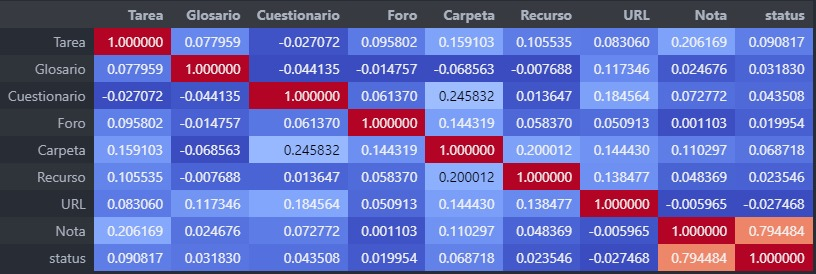
\includegraphics[width = 1 \textwidth]{Graphics/corr_dataset1.jpg}
    \caption{Matriz de correlación del \textit{Dataset} 1}
    \label{dataset1_corr}
\end{figure}  


En la figura \ref*{dataset1_corr} se muestra que las variables implicadas tienen muy poca relación entre ellas. El vínculo más importante es el que se establece entre cada una de las características y el estado final, ya que esto da una métrica de cuáles son los atributos que tienen mayor implicación 
en el desempeño del estudiante que es el estado final. El mayor coeficiente $0.090817$ perteneciente a la relación 
entre la variable \textbf{Tarea} y el estado final da una muestra de la poca conexión existente en las variables implicadas. Este resultado implica que utilización de la plataforma no es la correcta por parte de los estudiantes, así como existe poca rigurosidad por parte de los profesores a la hora de establecer una enseñanza en línea.  

A este \textit{dataset} se le aplicó 30 iteraciones del algoritmo Boruta en busca de encontrar las variables más importantes en la clasificación. El resultado fue el siguiente:   


\begin{figure}[htbp]
    \centering
    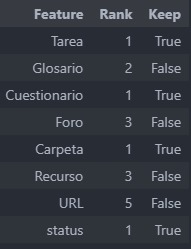
\includegraphics[height=5cm]{Graphics/boruta_dataset1.jpg}
    \caption{Resultado del algoritmo Boruta en el primer \textit{Dataset}}
    \label{boruta1}
\end{figure}   



En la figura \ref{boruta1} da como respuesta que se deben mantener los atributos: \textbf{Tarea}, \textbf{Cuestionario}, 
\textbf{Carpeta}, \textbf{URL}. Este resultado coincide con los mayores coeficientes de correlación de los atributos con el estado final del estudiante (figura \ref{dataset1_corr}). 
Además se muestra que el uso de los foros, glosarios y recursos no es bueno en este contexto.

En las figuras [\ref{dataset1_25}-\ref{dataset1_100}] se muestra una perspectiva diferente de los 5 modelos predictivos utilizados sin el filtrado de características
en términos de 4 medidas: exactitud (\textit{accuracy}), precisión (\textit{precision}), recuperación (\textit{recall}) y la medida f1.   





\begin{figure}[htbp]
    \centering
    \begin{minipage}[t]{0.50\textwidth}
        \centering
        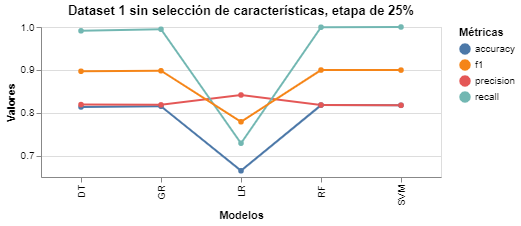
\includegraphics[width = \textwidth]{Graphics/dataset_1_25.png}
        \caption{Resultados del \textit{dataset} 1, etapa 25\%}
        \label{dataset1_25}
    \end{minipage}\hfill
    \begin{minipage}[t]{0.50\textwidth}
        \centering
        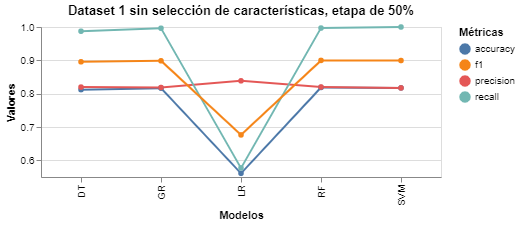
\includegraphics[width = \textwidth]{Graphics/dataset_1_50.png}
        \caption{Resultados del \textit{dataset} 1, etapa 50\%}
        \label{dataset1_50}
    \end{minipage}
\end{figure}

\begin{figure}[htbp]
    \centering
    \begin{minipage}[t]{0.50\textwidth}
        \centering
        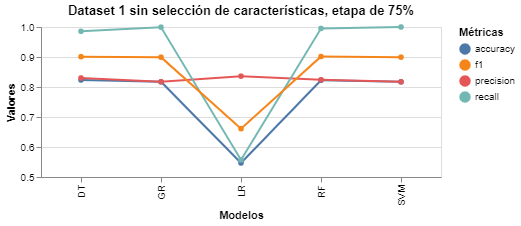
\includegraphics[width = \textwidth]{Graphics/dataset_1_75.png}
        \caption{Resultados del \textit{dataset} 1, etapa 75\%}
        \label{dataset1_75}
    \end{minipage}\hfill
    \begin{minipage}[t]{0.50\textwidth}
        \centering
        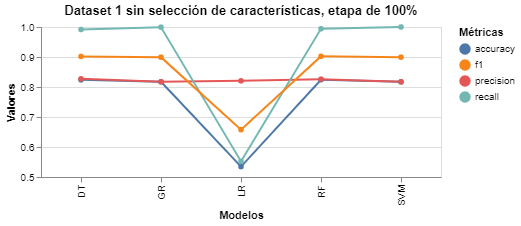
\includegraphics[width = \textwidth]{Graphics/datatset_1_100.png}
        \caption{Resultados del \textit{dataset} 1, etapa 100\%}
        \label{dataset1_100}
    \end{minipage}
\end{figure}  


De estos resultados se concluye:  
\begin{itemize}
    \item Primero, con un 25\% de progreso del curso, como se muestra en la figura \ref{dataset1_25}, la medida f1 más alta para 
    esta etapa promedió 0.899577 (89.9\%) por parte del algoritmo \textit{Random Forest}, sin embargo el modelo de Regresión Lineal presente la mayor precisión con 0.841331, además de ser el modelo mejor balanceado.
    \item En segundo lugar, en la figura \ref{dataset1_50} se muestra la etapa intermedia del 50\% del curso, no se muestran cambios relevantes en cuanto a las medidas en ninguno de los modelos, en este caso el Árbol de decisión logró la mejor medida f1 de 0.895660 y el algoritmo de Regresión Lineal la mayor precisión con 0.838568. .
    \item De manera similar en el 75\% de progreso como se observa en la figura \ref{dataset1_75} el modelo Regresión Lineal obtuvo la mejor precisión de 0.836072 y y el Árbol de Decisión la mayor medida f1 de 0.901137. 
    \item Por último, cuando se completó el curso como se muestra en la figura \ref{dataset1_100}, el Árbol de Decisión superó a los demás con una precisión de 0.827242 y una medida f1 de 0.902335. 
\end{itemize}

También se observa que en todas las etapas la recuperación es alta, esto significa que todos los modelos tienen la capacidad de encontrar de manera efectiva los verdaderos positivos en la predicción, cosa que puede ser perjudicial porque esto puede ser a expensas de aumentar el número de falsos positivos. Se propone aumentar el conjunto de datos, y añadir más estudiantes suspensos para mejorar este aspecto. 


En las figuras [\ref{dataset1_fs_25} - \ref{dataset1_fs_100}] se observa el comportamiento de todos los modelos con un filtrado de características luego de la selección con el algoritmo Boruta.

\begin{figure}[htbp]
    \centering
    \begin{minipage}[t]{0.50\textwidth}
        \centering
        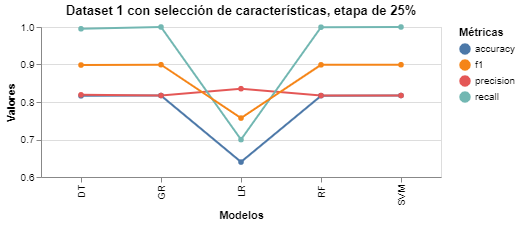
\includegraphics[width = \textwidth]{Graphics/dataset_1_fs_25.png}
        \caption{Resultados del \textit{dataset} 1 con filtro de características, etapa 25\%}
        \label{dataset1_fs_25}
    \end{minipage}\hfill
    \begin{minipage}[t]{0.50\textwidth}
        \centering
        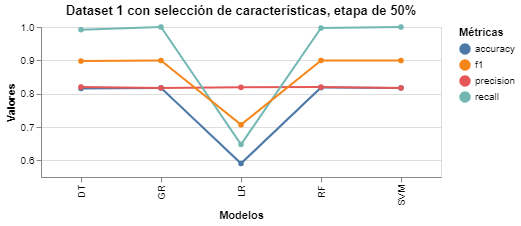
\includegraphics[width = \textwidth]{Graphics/dataset_1_fs_50.png}
        \caption{Resultados del \textit{dataset} 1 con filtro de características, etapa 50\%}
        \label{dataset1_fs_50}
    \end{minipage}
\end{figure}

\begin{figure}[htbp]
    \centering
    \begin{minipage}[t]{0.50\textwidth}
        \centering
        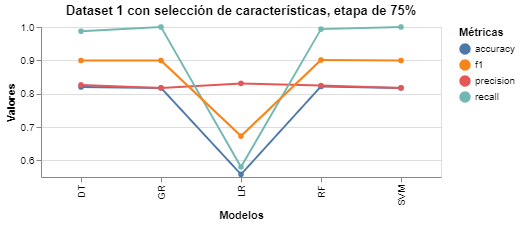
\includegraphics[width = \textwidth]{Graphics/dataset_1_fs_75.png}
        \caption{Resultados del \textit{dataset} 1 con filtro de características, etapa 75\%}
        \label{dataset1_fs_75}
    \end{minipage}\hfill
    \begin{minipage}[t]{0.50\textwidth}
        \centering
        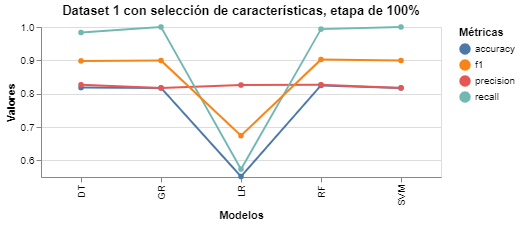
\includegraphics[width = \textwidth]{Graphics/dataset_1_fs_100.png}
        \caption{Resultados del \textit{dataset} 1 con filtro de características, etapa 100\%}
        \label{dataset1_fs_100}
    \end{minipage}
\end{figure}   

Como se puede apreciar no hubo cambios significativos con respecto al entrenamiento con todas las características.  Siendo el modelo Regresión Lineal nuevamente el de mejor precisión con respecto a los demás y el \textit{Random Forest} el de mejor medida f1. 


\subsection{Análisis del segundo \textit{dataset}}

\begin{figure}[htb]
    \centering
    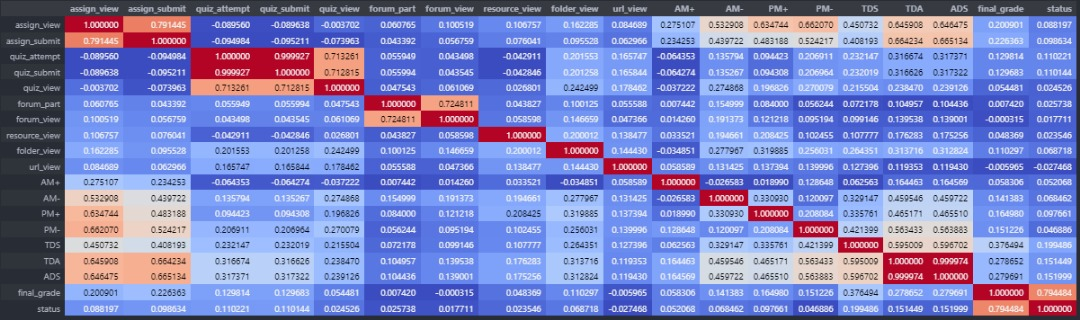
\includegraphics[width = 1 \textwidth]{Graphics/corr_dataset2.jpg}
    \caption{Matriz de correlación del \textit{Dataset} 2}
    \label{dataset2_corr}
\end{figure}  


En este conjunto de datos se tuvieron en cuenta otras variables como se muestra en la figura \ref{dataset2_view}. Con este cambio los coeficientes de correlación mejoraron con respecto al \textit{dataset} anterior, como se observa en la 
figura \ref{dataset2_corr} la mayor conexión con el estado final la alcanzan los atributos: TAD (\textit{total access days}, cantidad de días distintos en que el estudiante accedió al sitio) y 
ADS (\textit{access density score}, proporción entre TAD y el total del días de duración del curso), con 0.151449 y 0.151999 respectivamente. 
En general los coeficientes se mantienen bajos, pero este dataset da una perspectiva más amplia de lo que realiza un estudiante dentro de un curso.

Al aplicar el algoritmo Boruta nuevamente con 30 iteraciones, se produjo el siguiente resultado: 


\begin{figure}[htb]
    \centering
    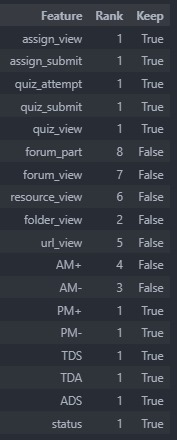
\includegraphics[height=6cm]{Graphics/boruta_dataset2.jpg}
    \caption{Resultado del algoritmo Boruta en el segundo \textit{Dataset}}
    \label{boruta2}
\end{figure} 

Como se muestra en la figura \ref{boruta2} las características más importantes coinciden con los atributos de mayor coeficiente de correlación con respecto al estado final. Además se vuelve a evidenciar que el foro y los recursos no son relevantes dentro de este contexto. 


Como con el conjunto de datos anterior, se entrenaron todos los modelos primeramente sin el filtrado de características y luego con los atributos relevantes.  


\begin{figure}[htbp]
    \centering
    \begin{minipage}[t]{0.50\textwidth}
        \centering
        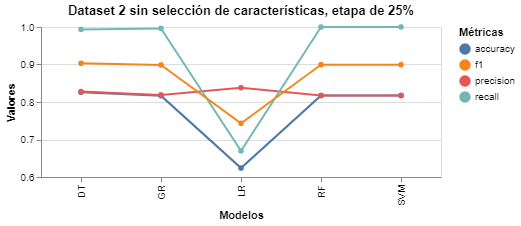
\includegraphics[width = \textwidth]{Graphics/dataset_2_25.png}
        \caption{Resultados del \textit{dataset} 2, etapa 25\%}
        \label{dataset2_25}
    \end{minipage}\hfill
    \begin{minipage}[t]{0.50\textwidth}
        \centering
        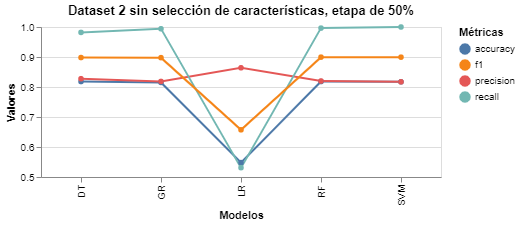
\includegraphics[width = \textwidth]{Graphics/dataset_2_50.png}
        \caption{Resultados del \textit{dataset} 2, etapa 50\%}
        \label{dataset2_50}
    \end{minipage}
\end{figure}

\begin{figure}[htbp]
    \centering
    \begin{minipage}[t]{0.50\textwidth}
        \centering
        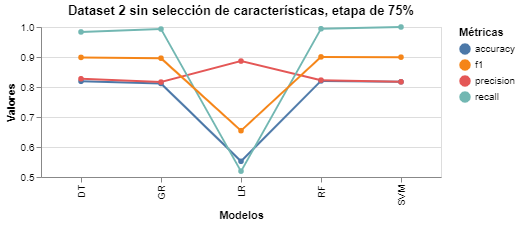
\includegraphics[width = \textwidth]{Graphics/dataset_2_75.png}
        \caption{Resultados del \textit{dataset} 2, etapa 75\%}
        \label{dataset2_75}
    \end{minipage}\hfill
    \begin{minipage}[t]{0.50\textwidth}
        \centering
        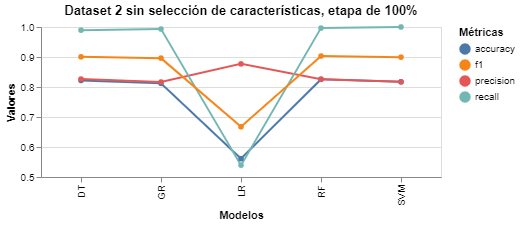
\includegraphics[width = \textwidth]{Graphics/dataset_2_100.png}
        \caption{Resultados del \textit{dataset} 2, etapa 100\%}
        \label{dataset2_100}
    \end{minipage}
\end{figure}

En las figuras [\ref{dataset2_25}-\ref{dataset2_100}] se muestran los resultados de cada modelo en cada etapa.  

De estos resultados se concluye:  
\begin{itemize}
    \item En el 25\% de progreso del curso, como se muestra en la figura \ref{dataset2_25}, la medida f1 más alta para 
    esta etapa promedió 0.903166 (90.3\%) por parte del algoritmo Árbol de Decisión, sin embargo el modelo de Regresión Lineal presenta la mayor precisión con 0.841331.
    \item En segundo lugar, en la figura \ref{dataset2_50} se muestra la etapa intermedia del 50\% del curso, no se muestran cambios relevantes, en este caso el \textit{Random Forest} logró la mejor medida f1 de 0.899510 y el algoritmo de Regresión Lineal la mayor precisión con 0.864092. 
    \item De manera similar en el 75\% de progreso como se observa en la figura \ref{dataset2_75} el modelo Regresión Lineal alcanzó la mejor precisión de 0.886431 y el \textit{Random Forest} la mayor medida f1 de 0.900394. 
    \item Por último, cuando se completó el curso como se muestra en la figura \ref{dataset2_100}, el algoritmo Regresión Lineal superó a los demás en cuanto a la precisión con una puntuación de 0.877038 y el \textit{Random Forest} tuvo la mejor medida f1 con 0.903177. 
\end{itemize}

Al igual que en el \textit{dataset} anterior la recuperación en todos los modelos excepto en el de Regresión Lineal, es muy cercana a 1, lo que vuelve a poner de manifiesto el mismo problema.

En las figuras [\ref{dataset2_fs_25} - \ref{dataset2_fs_100}] se observa el comportamiento de todos los modelos con un filtrado de características luego de la selección con el algoritmo Boruta en el segundo conjunto de datos.

\begin{figure}[htbp]
    \centering
    \begin{minipage}[t]{0.50\textwidth}
        \centering
        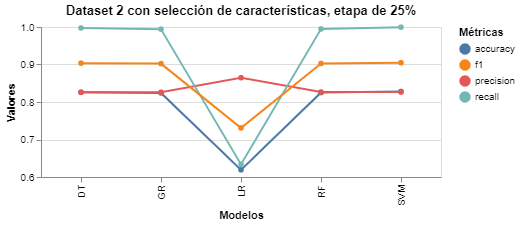
\includegraphics[width = \textwidth]{Graphics/dataset_2_fs_25.png}
        \caption{Resultados del \textit{dataset} 2 con filtro de características, etapa 25\%}
        \label{dataset2_fs_25}
    \end{minipage}\hfill
    \begin{minipage}[t]{0.50\textwidth}
        \centering
        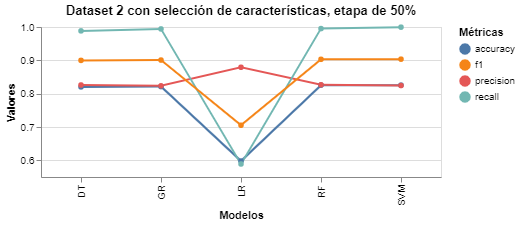
\includegraphics[width = \textwidth]{Graphics/dataset_2_fs_50.png}
        \caption{Resultados del \textit{dataset} 2 con filtro de características, etapa 50\%}
        \label{dataset2_fs_50}
    \end{minipage}
\end{figure}

\begin{figure}[htbp]
    \centering
    \begin{minipage}[t]{0.50\textwidth}
        \centering
        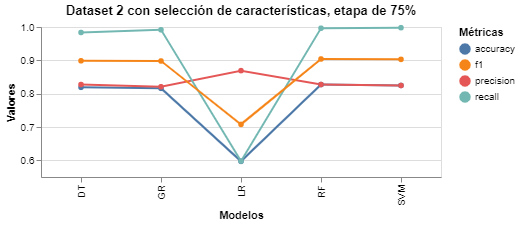
\includegraphics[width = \textwidth]{Graphics/dataset_2_fs_75.png}
        \caption{Resultados del \textit{dataset} 2 con filtro de características, etapa 75\%}
        \label{dataset2_fs_75}
    \end{minipage}\hfill
    \begin{minipage}[t]{0.50\textwidth}
        \centering
        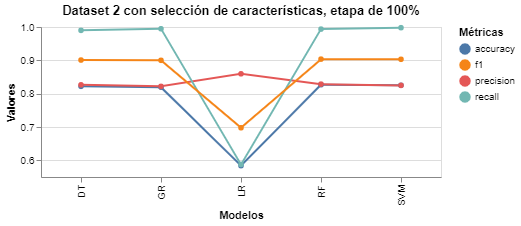
\includegraphics[width = \textwidth]{Graphics/dataset_2_fs_100.png}
        \caption{Resultados del \textit{dataset} 2 con filtro de características, etapa 100\%}
        \label{dataset2_fs_100}
    \end{minipage}
\end{figure}

Como se puede apreciar no hubo cambios significativos con respecto al entrenamiento con todas las características.  Siendo el modelo Regresión Lineal nuevamente el de mejor precisión con respecto a los demás y el \textit{Random Forest} el de mejor medida f1. 

De manera general el algoritmo Regresión Lineal es el más balanceado en cada una de las etapas para ambos datasets. Dentro del contexto de esta investigación este modelo es el mejor dado que a diferencia de los demás. 
Presenta valores de recuperación que oscilan entre los 0.5 y 0.7, que en este problema en 
particular de predicción académica es bueno, ya que eso significa que el modelo no hace énfasis en los estudiantes aprobados, y aún así logra una buena precisión a la hora de la evaluación. 


